\newpage

\section{Medições em laboratório}

\begin{figure}[h]
    \centering
    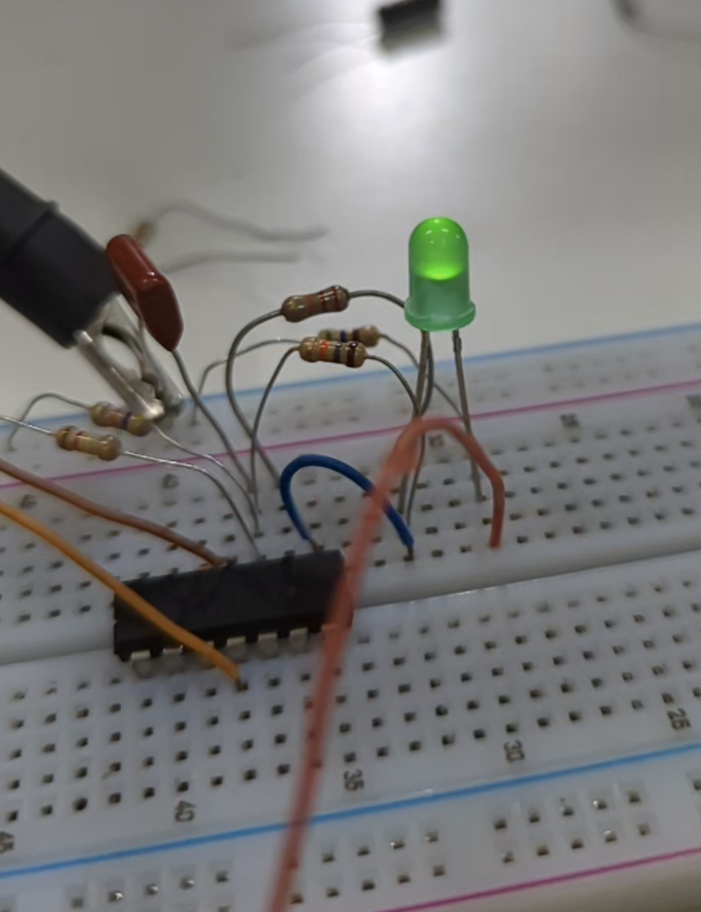
\includegraphics[width=0.3\columnwidth]{images/circuito_montado.png}
    \caption{Imagem do circuito montado em laboratório.}
\end{figure}

Nesta seção, são apresentados os detalhes e resultados das medições realizadas no experimento, com o objetivo de obter dados quantitativos para análise e validação dos resultados teóricos previamente obtidos.

\subsection{Exemplo 1}

\subsubsection{Componentes}

\begin{equation}
    \begin{aligned}
         & R_1 = 14890 \varOmega  \\
         & R_2 = 11758 \varOmega  \\
         & R_3 = 46890 \varOmega  \\
         & R_4 = 100380 \varOmega \\
         & R_5 = 551.1 \varOmega  \\
         & C = 10.4nF             \\
    \end{aligned}
\end{equation}


\subsubsection{$V_o (t)$}

\begin{figure}[H]
    \label{fig:ex2}
    \centering
    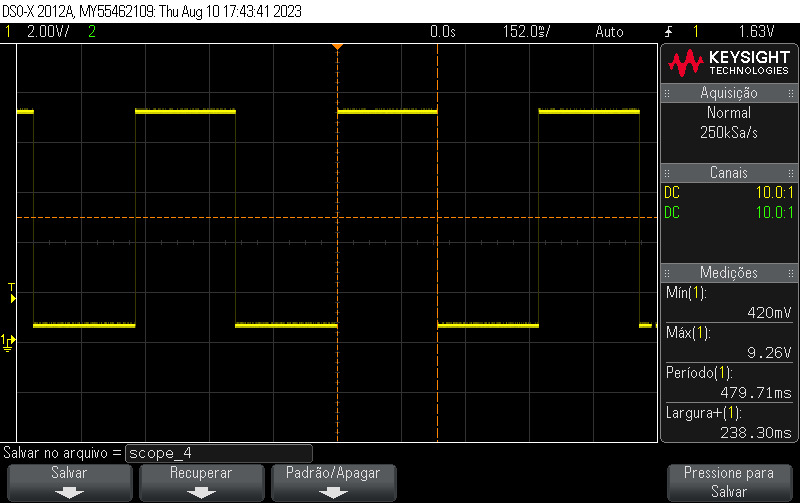
\includegraphics[width=0.7\columnwidth]{images/ex1_vo.png}
    \caption{Medição de $V_o(t)$ vista no osciloscópio para três períodos.}
\end{figure}

Da imagem obtemos os seguintes dados:

\begin{equation}
    \begin{aligned}
         & V_{m1} = 460mV \\
         & V_{m2} = 9.22V \\
         & T = 510.62ms   \\
         & kT =  255.31ms \\
    \end{aligned}
\end{equation}


\subsubsection{$V_c (t)$}

\begin{figure}[H]
    \centering
    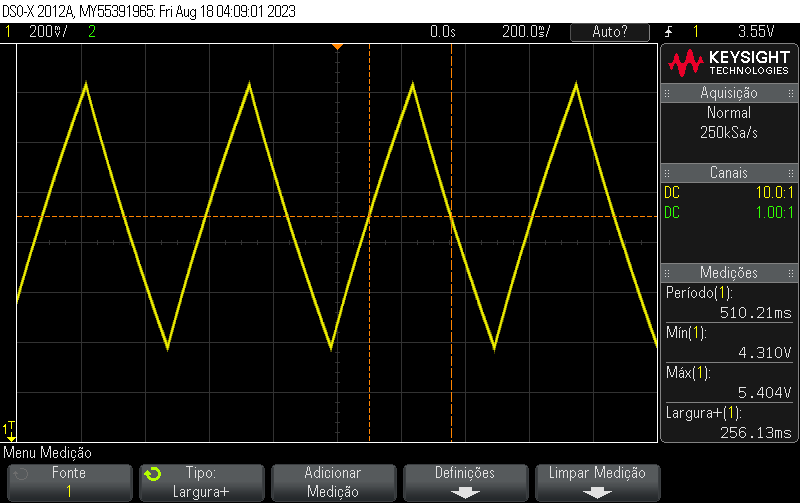
\includegraphics[width=0.7\columnwidth]{images/ex1_vc0.png}
    \caption{Medição de $V_c(t)$ vista no osciloscópio para três períodos.}
\end{figure}

Da imagem obtemos os seguintes dados:

\begin{equation}
    \begin{aligned}
         & V_{m1} = 4.31V  \\
         & V_{m2} = 5.404V \\
         & T = 510.21ms    \\
         & kT =  256.13ms  \\
    \end{aligned}
\end{equation}

\subsubsection{$V_{R5} (t)$}

\begin{figure}[H]
    \centering
    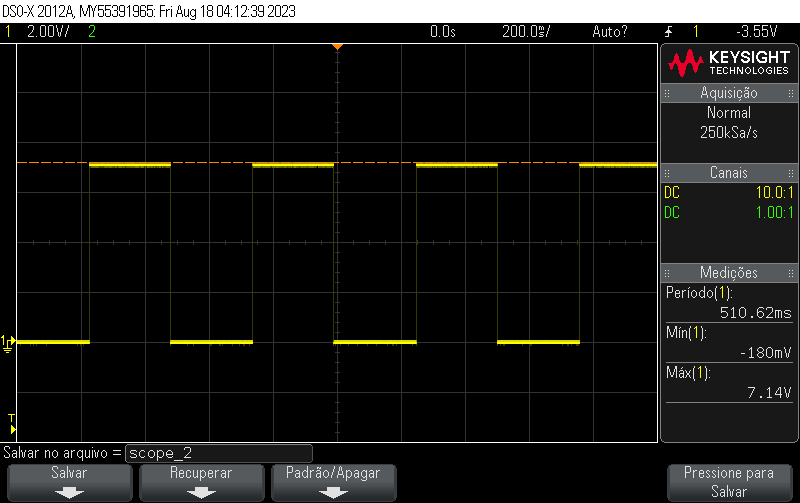
\includegraphics[width=0.7\columnwidth]{images/ex1_r5.png}
    \caption{Medição de $V_{R5}(t)$ vista no osciloscópio para três períodos.}
\end{figure}

Da imagem obtemos os seguintes dados:

\begin{equation}
    \begin{aligned}
         & V_{m1} = -180mV \\
         & V_{m2} = 7.14V  \\
         & T = 510.61ms    \\
         & kT =  255.3ms   \\
    \end{aligned}
\end{equation}

% adsda

\subsection{Exemplo 2}

\subsubsection{Componentes}

\begin{equation}
    \begin{aligned}
         & R_1 = 118950 \varOmega \\
         & R_2 = 46890 \varOmega  \\
         & R_3 = 17752 \varOmega  \\
         & R_4 = 21914 \varOmega  \\
         & R_5 = 551.1 \varOmega  \\
         & C = 101.16nF           \\
    \end{aligned}
\end{equation}


\subsubsection{$V_o (t)$}

\begin{figure}[H]
    \centering
    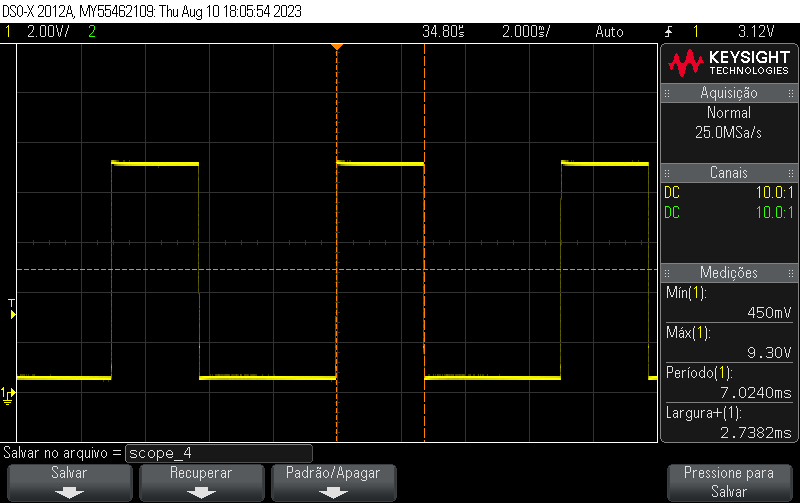
\includegraphics[width=0.7\columnwidth]{images/ex2_vo.png}
    \caption{Medição de $V_o(t)$ vista no osciloscópio para três períodos.}
\end{figure}

Da imagem obtemos os seguintes dados:

\begin{equation}
    \begin{aligned}
         & V_{m1} = 470mV \\
         & V_{m2} = 9.23V \\
         & T = 7.4435ms   \\
         & kT =  2.9ms    \\
    \end{aligned}
\end{equation}


\subsubsection{$V_c (t)$}

\begin{figure}[H]
    \centering
    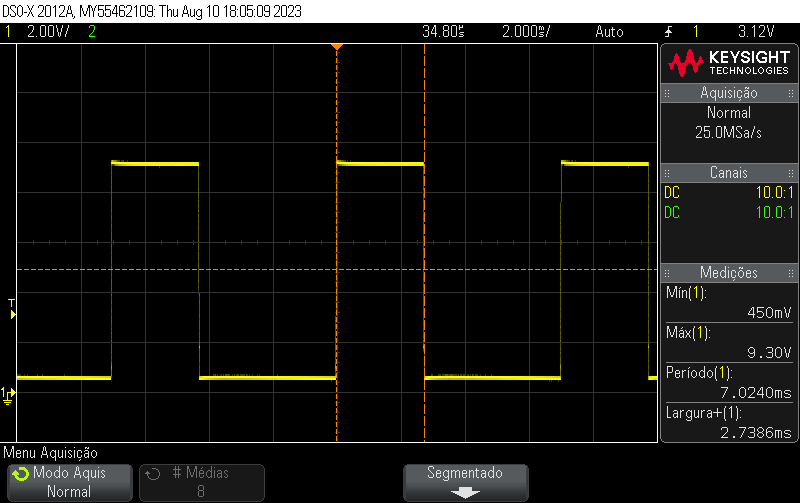
\includegraphics[width=0.7\columnwidth]{images/ex2_vc.png}
    \caption{Medição de $V_c(t)$ vista no osciloscópio para três períodos.}
\end{figure}

Da imagem obtemos os seguintes dados:

\begin{equation}
    \begin{aligned}
         & V_{m1} = 1.35V \\
         & V_{m2} = 7.14V \\
         & T = 7.4365ms   \\
         & kT =  2.91ms   \\
    \end{aligned}
\end{equation}

O valor do $kT$ foi obtido a partir de uma imagem que não se encontra aqui no relatório, ela está na pasta "images" que foi enviada junto com o relatório.

\subsubsection{$V_{R5} (t)$}

\begin{figure}[H]
    \centering
    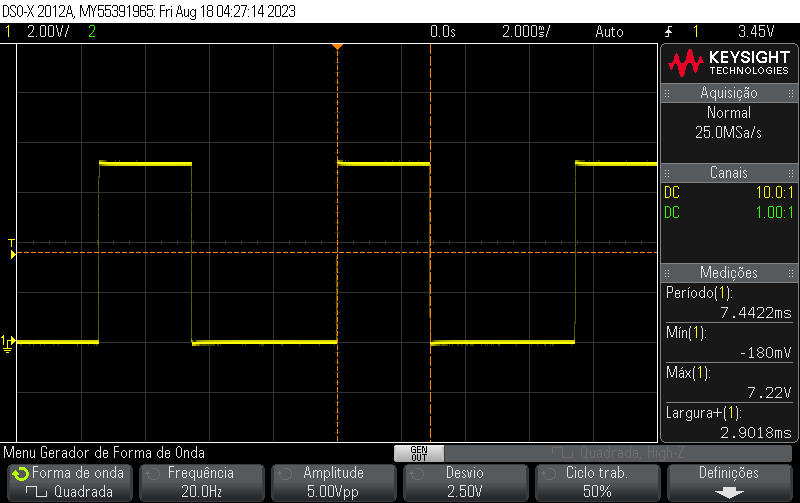
\includegraphics[width=0.7\columnwidth]{images/ex2_r5.png}
    \caption{Medição de $V_{R5}(t)$ vista no osciloscópio para três períodos.}
\end{figure}

Da imagem obtemos os seguintes dados:

\begin{equation}
    \begin{aligned}
         & V_{m1} = -180mV \\
         & V_{m2} = 7.22V  \\
         & T = 7.4422ms    \\
         & kT =  2.9018ms  \\
    \end{aligned}
\end{equation}